\chapter{Danske Bank}

Danske bank is the largest bank in Denmark \cite[p.~38]{danske_bank_setting_up_in_denmark}, with 2.7 million personal customers, 238,000 small and medium-sized business customers and 1,700 corporate and institutional customers, across the Nordic countries and in Northern Ireland. Danske bank offers a wide range of banking services for Danish and international customers, promising highly available and feature rich digital solutions. Danske bank is active in many sectors within the fields of banking, providing comprehensive digital solutions within each, resulting in several high-end digital solutions. Current solutions include comprehensive web solutions, tablet and smarthphones applications for personal banking and a leading mobile payment application with more than 400.000 transactions daily. Danske bank prioritizes being on the technological forefront, deeming it highly important for customer satisfaction and retainment stating the following on their website\cite{danske_bank_our_essence}:

\tquote{We have a constant focus on improving our advisory services and developing unique digital products. Our goal is to give our customers the best possible advice and provide them with seamless digital solutions. By continuously developing our offerings and introducing new and innovative tools, we aim to create value for all our customers – from making daily payments easy for our private customers to supporting our large, corporate customers in developing their business}{Danske bank}{2017}

\note{Developing, expanding and maintaining a so comprehensive digital infrastructure is very demanding and complex. 
Being the first Danish bank to release mobile banking and mobile payment on smartphones 
Complex infrastructure
Data handling
1 mill transactions}

Danske bank has a high amount of existing systems, having active in-house software development projects running for more than 30 years. Danske bank is a big and complex organisation, which is reflected in their software infrastructure, that consists of a diverse and extensive range of software systems of varying size. Many of the earlier developed software projects are labelled by developers as being 'legacy systems' referred to with equal amounts of respect and awe. As some of these legacy systems have been extensively utilized in a steady growing amount of new applications, developers have faced many challenges with high coupling and loss of cohesion. The following chapter will present and analyse one of these legacy systems, that is essential to one of the business areas within Danske bank, more specifically agreements for business customers and their access to banking services.

\section{The shared database}
Danske bank has a multitude of applications sharing a common database layer, that contains a wide variety of information about newly created and existing business customers and their access privileges to services within Danske bank. Development of the shared database was according to Danske bank started in 1991, where dependent applications were integrated closely with the database. Each application had the necessary logic for manipulating the database according to it's needs. Based on problems with a high amount of duplicated code across the expanding sets of interacting applications Danske bank initiated a reiteration of the shared database architecture in 2006. 

An small part of the current and enormous architecture can be seen on Figure \ref{fig:danske_bank_shared_database}, the architecture can be divided into three layers: Application layer, Database access layer and a Database layer. The application layer consists of many diverse applications, each utilizing the common database either through a specific access service or by directly communicating with the database. The database is mainly accessed through a multitude of different services, in the database access layer, these services act as interfaces to the database, ensuring that data is created, read, updated and deleted according to the specific context. The database layer consists of a resource intensive IBM DB2 relation database management system (RDMS), hosting a SQL database. 

\note{The database effectively sits as a integration tool for the multitude of dependent applications.}

\begin{figure}[!htb]
  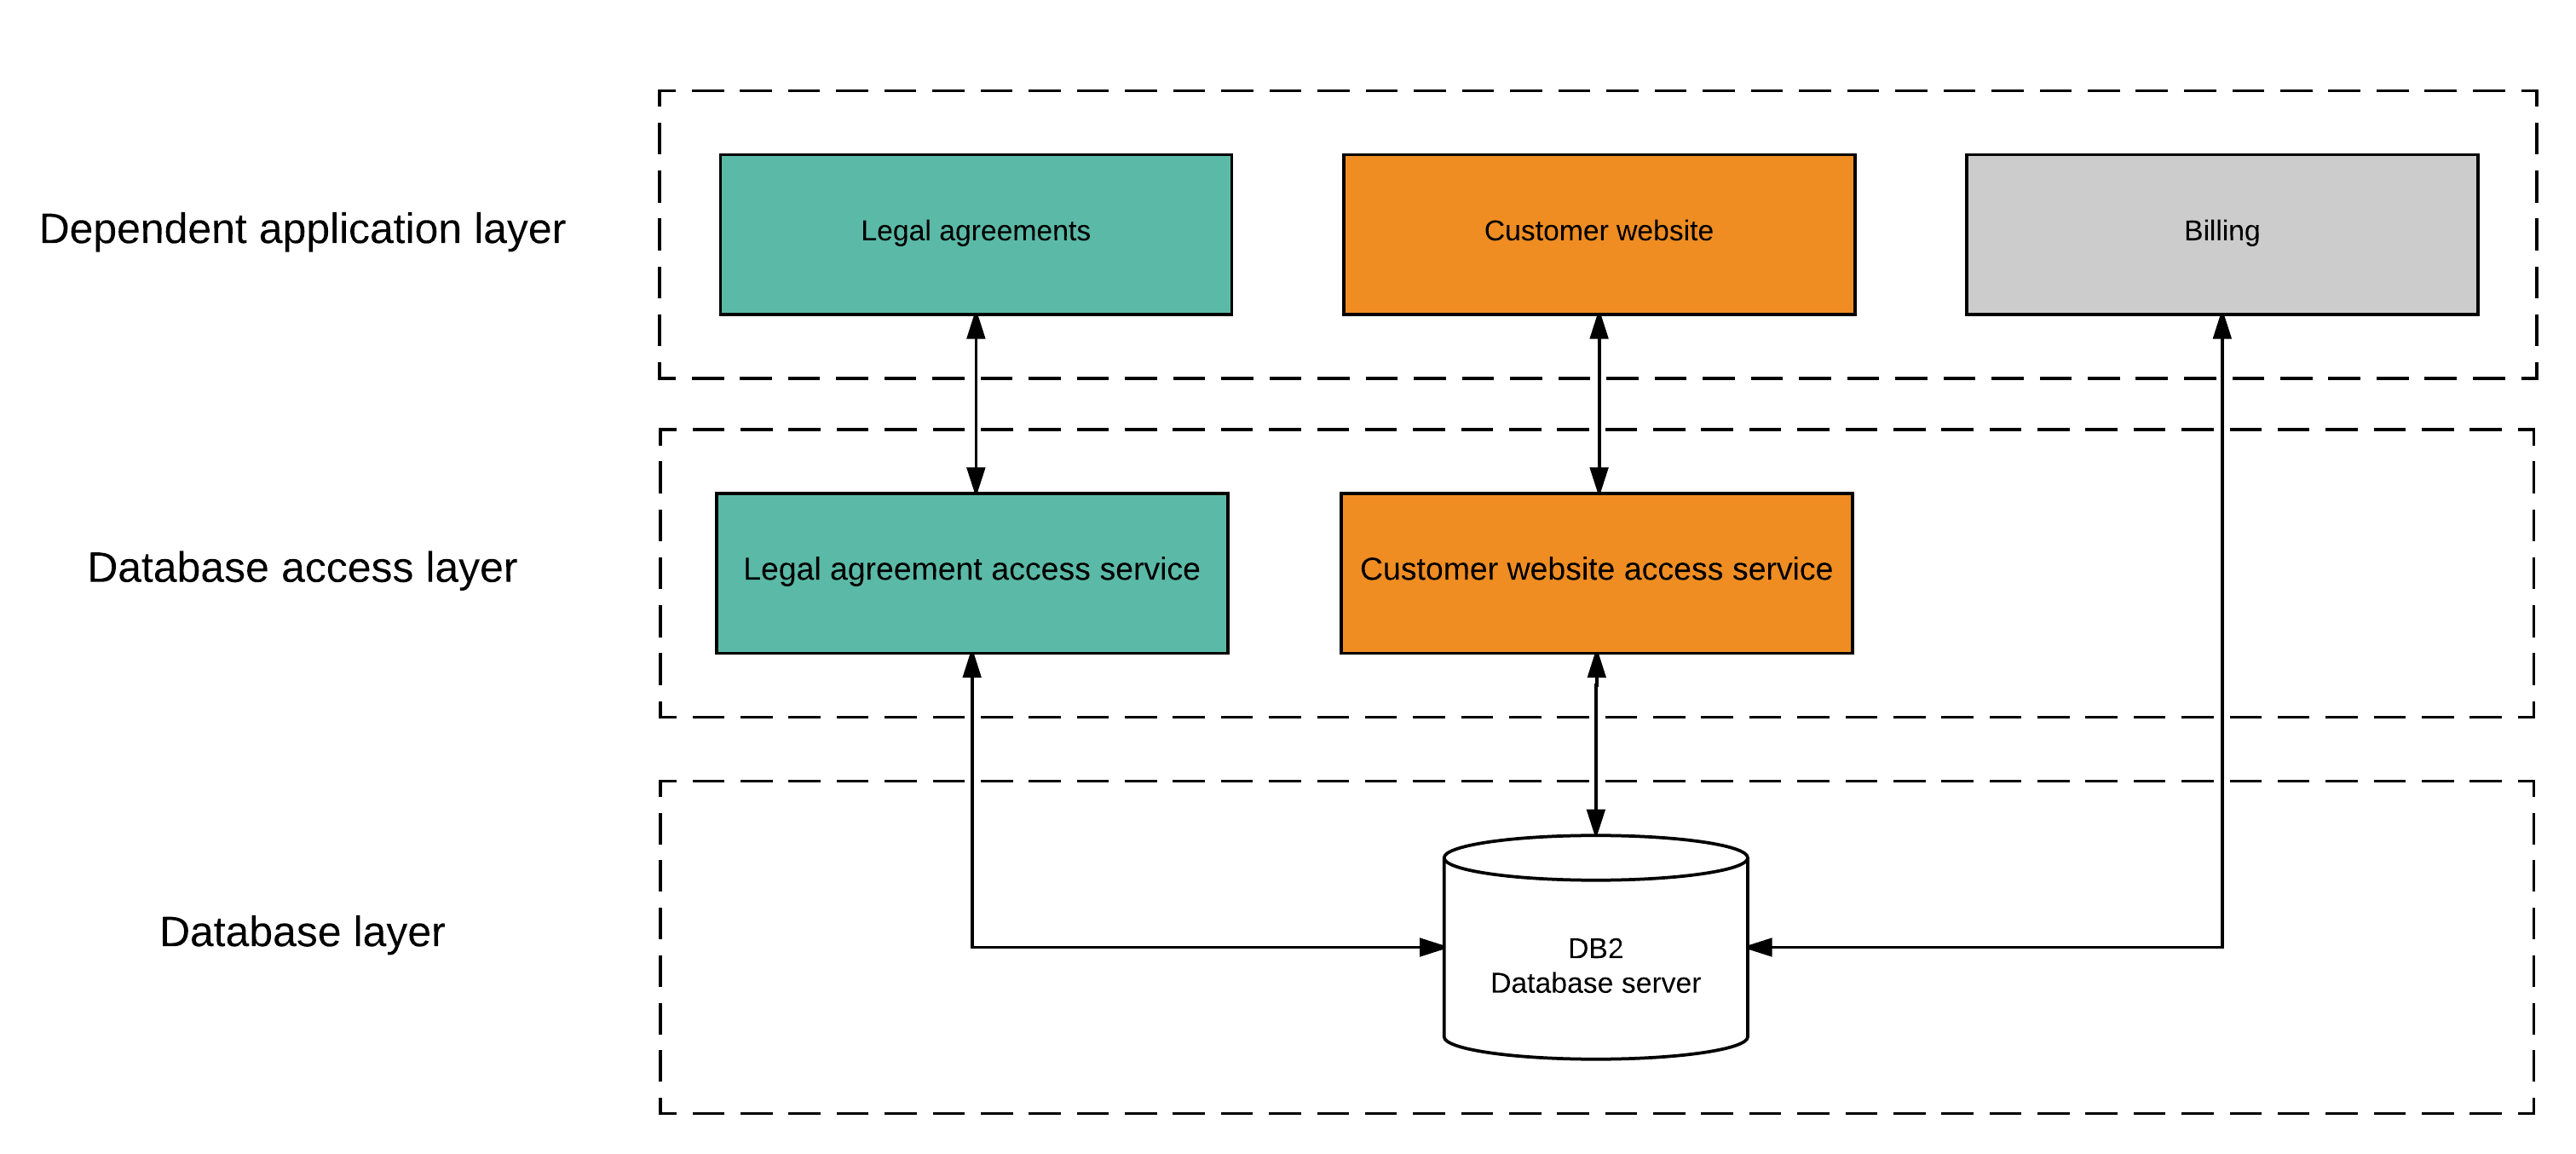
\includegraphics[scale=0.14]{danske_bank_shared_database}  
  \caption{Datbase integration architecture}
  \label{fig:danske_bank_shared_database}
\end{figure}


Even though Danske bank has tried to combat some of the issues with a shared database architecture, there is still inherently many problems with the architecture. 

\subsection{Challenges with a shared database}
The shared database is a very common form of integration, and according to Newman the most common one\cite[p.~41]{newman2015microservices}. A database integration starts out very simple and is quickly established, but with time becomes rigid.

\subsubsection{Single point of failure}
Each consumer is highly reliant on a correct and running database. All consumers are communicating with the same database, inferring a very high responsibility on each consumer, a incorrect implementation could cause the database to collapse, due to malformed or a high amount of requests from a single or several consumers.
A high amount of applications are dependent on the singular database, the lack of redundancy would cause a complete stop to the many applications dependent on the database, if it was ever to crash.

\subsubsection{High coupling}
Each consumer without a database access layer is highly couple to the database, making changes to the database structure incur changes in all directly linked consumers implementation.

\subsubsection{Loss of cohesion}
By having several database access layers and dependent applications directly interacting with the database, the logic required to perform common operations on the database is duplicated. This infers a big overhead if a bug is discovered within this common logic, making it necessary to update several code bases with the same fix.

\note {

\subsection{Pace of change}

\subsection{Team Structure}

\subsection{Security}

\subsection{Technology}

}

\note{
\subsection{Where Danske bank want to go}
Distribute responsibility, each consumer wanting to subscribe to the data source, has it's own representation of the data, moving responsibility from the single database to a consumer database. Adding more consumers does hereby not introduce risk on all other consumers, by burdening a central database.

A more scalable solution, where an unlimited number of consumers can be added, solving limitations in the current implementation. Not limiting database implementation, making it possible to swap individual parts of the system without incurring change on the rest of the system.
}

\note{

\subsection{Meeting with Thomas}
Development of this system began in 1991, where integration through a database was very common. Each dependent application had their own approach to doing CRUD commands directly on the database, validating data before creating new rows, implementing SQL statements for the different CRUD operations. 

The database exists within a system that lies centrally as a dependency for many applications. The system contains many different applications, from legacy to more newly developed applications, these applications control incoming requests, validate new data and serve aggregated data from the database. Each application has it's own implementation of all actions on the central database.

Later the integration was redone with interfaces, to ensure that applications communicated correctly with the database, making it possible to survey usage of it as well.

\subparagraph{Amount of dependent applications}
Many applications are dependent on the central database, more than 30 systems that consist of more than 50 applications each. 

\subparagraph{Interface}
The systems mainly communicate with the central database through communication interfaces, but some legacy applications still communicate directly with the database.
Many different interfaces are implemented, among others consisting of: mainframe modules and a variety of API approaches.

\subparagraph{Read/Write ratio}
There are no current figures on read/write ratio on the database, Thomas estimates that there is a 100000/1 read to write ratio. Operations on the database are not evenly distributed, some parts of the database are utilized more than others.


\subparagraph{Problems}
Each application in the central system has it's own implementation of all transactions on the database, inferring a high level of code duplication with many basic reoccurring transactions. When correcting or updating one of the transaction instances, similar implementations must be updated, sometimes covering more than hundred different implementations.

 implementation of a specific transaction is discovered, the 
}

\note{
\begin{quote_highlight}
\textbf{The Shared Database:} By far the most common form of integration that I or any of my colleagues see in the industry is database (DB) integration [...] This is really simple when you first think about it, and is probably the faster form of integration to start with [...] but it's one fraught with difficulties \cite[p.~41]{newman2015microservices}
\end{quote_highlight}


Access Control layer(proxy) description:
\url{https://www.3scale.net/2015/05/how-to-load-test-and-tune-performance-on-your-api-part-ii/}\\
\url{https://medium.com/netflix-techblog/optimizing-the-netflix-api-5c9ac715cf19}\\
\url{https://www.nginx.com/resources/wiki/}\\

\say{The Group offers Danish and international customers a wide range of services in the fields of banking, mortgage finance, insurance, leasing, real-estate brokerage and asset management} 


Danske bank has been in constant development, modernizing existing and creating new systems, with a focus on 
focusing on creating highly available, consistent and scalable solutions.


No JOINS on table, too slow


Properly not a very good Normalization form


In need of something that can server a lot of reads


External parties view and bind internal implementation

Logic associated with interpreting and changing data is spread out, if some logic contains a bug or the database is changed, it infers changes multiple places, removing cohesion}